% !TEX root = main.tex
% !TEX encoding = UTF-8

\chapter{Preparation}

This chapter discusses two tools we used in this paper, SystemBuilder and Neural Network Console.

\section{SystemBuilder}\label{sec:SystemBuilder}
% \section{High-Level Synthesis Using SystemBuilder}\label{sec:SystemBuilder}
% \section{Design on SystemBuilder}

For the convenience of development for the FPGA, we used a system-level design toolkit named SystemBuilder. SystemBuilder is a toolkit that abstracts the interface between hardware and software, such as a device interface and bus interface. Due to such abstraction, a designer can have better productivity by eliminating the need to do such low-level designs themselves.

In SystemBuilder, we name processes that run either hardware or software as functional units. As a result of the interface's abstraction, SystemBuilder provides four communication channels between functional units. We name these channels as a communication primitive. Since a functional unit could be either hardware or software, these primitive can also be used between hardware and software or between hardware and hardware, or between software and software.

A Designer should develop functional units and define a connection between units using the provided communication primitive. A unit will be implemented either a hardware or software process based on a system specification that a designer defined. We will discuss more details of a design description in section \ref{sec:design_description}.

SystemBuilder then generates RTL hardware, RTOS-specific software, and the interface of these. SystemBuilder executes an external tool for synthesizing. Since SystemBuilder does partitioning of hardware and software, a designer can now efficiently explore hardware/software partitioning.

We will discuss the detail of the synthesis used in SystemBuilder in section \ref{sec:synthesis}. In section \ref{sec:cosimulation}, we will explain a co-simulation feature that SystemBuilder provides.
 To summarize, we will discuss the entire workflow in section \ref{sec:workflow}.

\subsection{Design description} \label{sec:design_description}
A designer should create the following files to use SystemBuilder.
\begin{itemize}
  \item Functional units written in C language.  % a set of processes running concurrently
  \item System DeFinition (SDF) file. This is a description of a design target. \Figref{fig:eg_sdf} is an example of the SDF file we designed in the case study. Due to space limitations, this figure contains only part of the file.

    An SDF file includes the following information:
    \begin{itemize}
  \item A partitioning scheme of functional units.
    \begin{quote}
      A partitioning scheme corresponds to line 3--7 in \Figref{fig:eg_sdf}. The figure declares `topmod' as a software process and the rest of the units as hardware processes.
    \end{quote}
  \item A number and names of communication primitives.
    \begin{quote}
      It corresponds to line 11--21 in \Figref{fig:eg_sdf}. It declares seven `BlockingChannel' and one `MemoryChannel'.
    \end{quote}
  \item Connection relations between functional units and communication primitives.
    \begin{quote}
        It corresponds to line 23--39 in \Figref{fig:eg_sdf}. Under each functional unit (process), it declares the relations with communication primitive. For example, in line 34--37, primitive `conv1\_mpool1' is declared as an input, and primitive `mpool1\_conv2' is declared as an output of process `mpool1'.
    \end{quote}
    \end{itemize}
\end{itemize}

SystemBuilder reads these files and follows the steps presented in section \ref{sec:workflow}.

\begin{figure}[tbp] % option htbp
  \centering
  \lstinputlisting[
    language=Verilog,
    linerange={1-39},
    % firstnumber=,
  ]{"src/sp_hw.yaml"}
  \caption{Example of System DeFinition file}
  \label{fig:eg_sdf}
\end{figure}

\begin{figure}[tb]
\centering
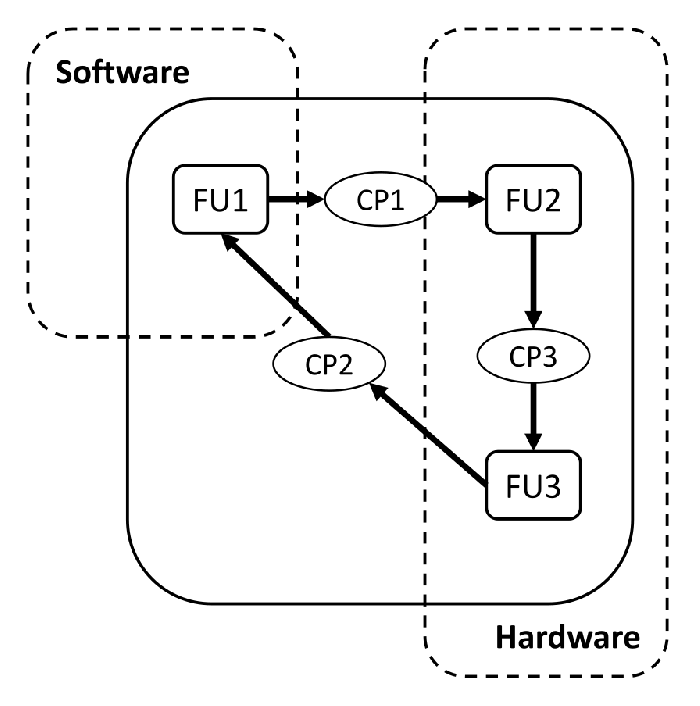
\includegraphics[width=0.49\textwidth]{example_partioning.eps}
\caption{Example of partitioning Functional Units}
\label{fig:example}
\end{figure}

\subsection{Partitioning}\label{sec:partitioning}
A designer using SystemBuilder should define a partition scheme in SDF File.
This means a designer can decide whether to implement functional units in hardware or software. For example, in \Figref{fig:example}, unit 1 is partitioned as a software process, units 2 and 3 as hardware processes.
To test another partitioning scheme, a designer has only to edit an SDF file and rerun SystemBuilder. In this way, a designer can efficiently explore a partition scheme of hardware/software. To test an implementation works as expected, a designer can run a co-simulation.
A Designer can test an implementation even faster by building all functional units as software. Since emulating software is much faster than simulating hardware, it is expected to be more efficient than running co-simulation. Co-simulation/simulation is discussed in section \ref{sec:cosimulation}.

\subsection{Functional Units (FU)}
As discussed in section \ref{sec:partitioning}, a designer can decide whether to implement a functional unit in hardware or software. However, there is a limitation. SystemBuilder uses an external high-level synthesis tool.
It means a functional unit to be implemented as a hardware process must be subjected to the external HLS tool's limitation.
On the contrary, a unit to be implemented as a software process does not have those limitations. It means that all units can be built as a software process, and it allows to test a design at a functional level.

\subsection{Communication Primitives}\label{sec:communication_primitives}
SystemBuilder supports four communication primitive as follows.

\begin{description}
  \item [Non-Blocking Communication Primitives (NBC)]\mbox{}\\
    NBC corresponds to a shared variable in software and a register in hardware.
  \item [Blocking Communication Primitives (BC)]\mbox{}\\
    BC corresponds to OS's communication feature in software and a FIFO in hardware. Access is executed by blocking in one direction.
  \item [Memory Primitives (MEM)]\mbox{}\\
    MEM corresponds to a global array in software and a dual-port memory in hardware. Access is executed by non-blocking.
    It is possible to implement a memory primitive as shared memory. In order to implement as shared memory, shared memory must be declared in an SDF file.
  \item [PreFetch BC (PFBC)]\mbox{}\\
    PFBC is a memory designed between external memory and hardware process. The purpose of PFBC is to hide latency while reading external memory. PFBC reads the bulk of data from external memory and provides fast internal memory to hardware processes connected. PFBC uses shared memory only available for the software process side; therefore, shared variables must also be declared separately.
\end{description}

These primitives can be accessed as a C language function when designing a unit.

\subsection{Synthesis} \label{sec:synthesis}
SystemBuilder takes SDF and C programs as an input and generates files for software, hardware, and interface.
% \subsubsection{Partitioning}

\subsection {Software Synthesis}
Software synthesis takes place by a compiler. It will be compiled as software running on either ITRON \cite{sakamura1987itron} or AUTOSAR-CP \cite{autosar}. Communication primitives between a software process are also implemented as software.

\subsection{Hardware Synthesis}\label{sec:hwsynthesis}
A hardware process and communication primitives between them will be synthesis as hardware. SystemBuilder uses a commercial tool to synthesis hardware processes. SystemBuilder supports the following HLS tool.

\begin{itemize}
    \item eXCite
    \item CyberWorkBech\cite{waka}
    \item Vivado HLS\cite{vivadohls}
\end{itemize}

These HLS tools support various optimization techniques such as:

\begin{itemize}
  \item Pipelining the loop to implement the operations in a loop in a concurrent manner.
  \item Unrolling the loop to exploit parallelism between loop iterations.
  \item Expanding the array signal into the individual variable.
  \item Unrolling multi-dimensional array by a dimension designer configured.
  \item Inlining the function.
\end{itemize}

In order to take advantage of these features, a designer is required to develop processes with this in mind. We had a brief compare test of pipelining the network's loop statement represented in \Tabref{tab:result} and \Tabref{tab:result2}.

\subsection{Interface Synthesis}
SystemBuilder automatically generates a hardware/software interface based on the SDF file. For the software, the device driver is generated. The device driver includes access functions, interrupt handlers, and semaphores for synchronization between hardware and software. For the hardware, the interface circuit described in HDL is generated. This interface includes glue logic that allows accessing the bus and the circuit that corresponds to communication primitives such as buffer or memory. The glue logic has an interface to a generic bus named VBUS. Therefore, SystemBuilder generates a circuit that converts protocol to connect VBUS.

\subsection{Command} \label{sec:command}
This subsection discusses the actual commands for synthesizing.

SystemBuilder provides `\texttt{SysGen}' command to synthesis the system. `\texttt{SysGen}' has the following options \cite{man:systembuilder}.

\begin{itemize}
  \item Specify the SDF file.
    \begin{description}
      \item[\texttt{-sdfy \textit{<SDF file>}}] Specify the YAML format of the SDF file.
      \item[\texttt{-sdf \;\;\textit{<SDF file>}}] Specify the sdf format of the SDF file.
    \end{description}
  \item Specify the synthesis method.
    \begin{description}
      \item[\texttt{-nobs}] Specify to not to perform high-level synthesis.
      \item[\texttt{-dobs}] Specify to perform high-level synthesis.
      \item[\texttt{-csim}] Specify to print C language level simulation.
    \end{description}
  \item Specify high-level synthesis tool.
    \begin{description}
      \item[\texttt{-bst <HLS tool name>}]
    \end{description}
  \item Specify the target board.
    \begin{description}
      \item[\texttt{-s <board name>}]
    \end{description}
  \item Specify the RTOS for running software processes.
    \begin{description}
      \item[\texttt{-os <itron or atk>}]
    \end{description}
  \end{itemize}

  `\texttt{SysGen}' commands synthesis the interface and hardware processes. It also generates `\texttt{Makefile}' for software compiles.


\subsection{Co-simulation} \label{sec:cosimulation}
To test a design, SystemBuilder supports hardware and software co-simulation. It runs RTOS emulator and RTL simulators and then coordinating them to perform co-simulation. It connects the RTOS emulator and RTL simulator by a program named device manager. The device manager runs on the host computer then connects to the RTOS emulator using an inter-process communication function from the host pc. While the RTOS emulator tries to communicate with the RTL simulator, the device manager sends a signal to the RTL simulator. The device manager uses Foreign Language Interface (FLI) to connect VBUS to the RTL simulator.

SystemBuilder supports running software processes either on QEMU or directly from the host computer. Functional Units that run on RTOS are compiled and linked with the RTOS model. Next, SystemBuilder generates an object code directly executable on the host computer \cite{honda2004rtos}. Due to native support, co-simulation speed is much faster than other simulators that simulate at the instruction-set level. In this paper, we used QEMU for the RTOS emulator and Questa Sim for the RTL simulator.

The benefit of running co-simulation is that designer can debug hardware processes. For example, a designer can observe a waveform of signals. \Figref{fig:eg_waveform} is an example of a waveform. In this figure, we can observe signals and variables.

\begin{figure}[tbp]
  \centering
  \includegraphics[width=0.99\linewidth]{questa_sim_wave.png}
  \caption{Waveform observed in Questa Sim}%
  \label{fig:eg_waveform}
\end{figure}


\subsection{Report from a HLS tool}\label{sec:report}

As a result of a high-level synthesis of hardware processes, several HDL files are created. To implement this result to the FPGA, logic synthesizing is required. At this time, the SystemBuilder requests the HLS tool to print several design reports. Design reports contain various information such as BRAM usage and LUT usage. \Tabref{tab:eg_memory} is an example of a memory usage report from Vivado. This table shows the BRAM usage of the design out of the RAM on the board. \Tabref{tab:eg_lut} is an example of LUT usage report. We can know the logic circuit size by LUT as logic usage. LUT usage can be an indicator of design efficiency.

\begin{table}[tbp]
  \centering
  \caption{Example of memory usage report}
  \label{tab:eg_memory}
  \begin{tabular}{|l|r|r|r|r|}
    \hline
Site Type         & Used & Fixed & Available & Util\% \\
\hline
Block RAM Tile       & 44.5 &     0 &       140 & 31.79  \\
\quad RAMB36/FIFO*   &   41 &     0 &       140 & 29.29  \\
\qquad RAMB36E1 only &   41 &       &           &        \\
\quad RAMB18         &    7 &     0 &       280 &  2.50  \\
\qquad RAMB18E1 only &    7 &       &           &        \\
\hline
  \end{tabular}
\end{table}

\begin{table}[tbp]
  \centering
  \caption{Example of LUT usage report}
  \label{tab:eg_lut}
  \begin{tabular}{|l|r|r|r|r|}
    \hline
                 Site Type                 &  Used & Fixed & Available & Util\% \\
\hline
Slice                                      &  3858 &     0 &     13300 & 29.01  \\
\quad  SLICEL                                   &  2587 &     0 &           &        \\
\quad  SLICEM                                   &  1271 &     0 &           &        \\
LUT as Logic                               &  9675 &     0 &     53200 & 18.19  \\
\quad  using O5 output only                     &     3 &       &           &        \\
\quad  using O6 output only                     &  7520 &       &           &        \\
\quad  using O5 and O6                          &  2152 &       &           &        \\
% LUT as Memory                              &   420 &     0 &     17400 &  2.41  \\
% \quad  LUT as Distributed RAM                   &   160 &     0 &           &        \\
% \qquad    using O5 output only                   &     0 &       &           &        \\
% \qquad    using O6 output only                   &    80 &       &           &        \\
% \qquad    using O5 and O6                        &    80 &       &           &        \\
% \quad  LUT as Shift Register                    &   260 &     0 &           &        \\
% \qquad    using O5 output only                   &     1 &       &           &        \\
% \qquad    using O6 output only                   &   231 &       &           &        \\
% \qquad    using O5 and O6                        &    28 &       &           &        \\
\hline
  \end{tabular}
\end{table}




\subsection{Workflow} \label{sec:workflow}

\begin{figure}[tb]
\centering
\includegraphics[width=0.66\textwidth]{workflowv2.eps}
\caption{Workflow inside SystemBuilder.}
\label{fig:systembuilder}
\end{figure}

In summary, we represent the workflow inside SystemBuilder in this section. \Figref{fig:systembuilder} and the following steps are an overview of workflow inside SystemBuilder.

\begin{enumerate}
    \item SystemBuilder read SDF Files and determines a partition scheme of functional units.
    \item SystemBuilder synthesis the interface between hardware and software.
    \item For software, a compiler compiles functional units with the device driver generated in step 2.
    \item For hardware, HLS Tool synthesis the code to HDL files.
    \item Users now can choose whether to run co-simulation or implement the results to FPGA.
    \begin{description}
    \item [Co-simulation] This process is described in section \ref{sec:cosimulation}.
    \item [FPGA] Logic synthesizer synthesis the HDL file created and device interface generated in step 2. This process generates design reports discussed in section \ref{sec:report}.
    \end{description}
\end{enumerate}

\section{Neural Network Console} \label{sec:nnc}

\begin{figure}[tbp]
  \centering
  \includegraphics[width=0.99\linewidth]{network_sample.png}
  \caption{Example of designing a neural network in NNC}%
  \label{fig:network_sample}
\end{figure}

A Designer can develop a network via GUI in NNC. \Figref{fig:network_sample} is an example of a network designed using NNC. As shown in this figure, NNC visualizes which layers are used in what order, from input to output.

% This section will cover the layers of NNC used in this paper. We will discuss the behavior of layers and properties. For some layers, we will also discuss the behavior at the source code level to better understand its behavior.
% the layers of NNC used in this paper. We will cover
% We will discuss the behavior of layers and properties.

This section will cover the behavior of FixedPointQuantize, convolution, affine layers of NNC. We will also discuss the behavior at the source code level to understand layers' behavior better. The source code referenced in this section is Neural Network Libraries' code, which NNC is built on.

% Neural Network Console is built on the Neural Network Libraries \cite{sony-nnabla}. This Libraries provides Python API built on the C++11 core. source code of this C+11 core.

% Neural Network Console is built on the Neural Network Libraries \cite{sony-nnabla}. This Libraries provides Python API built on the C++11 core. \Figref{fig:fixedpointquantize} is a part of source code of this C+11 core.

\subsection{FixedPointQuantize}
FixedPointQuantize layer performs linear quantization. This layer requires the following properties \cite{man:nnc}.

\begin{quote}
\begin{description}
  \item[Sign] Specify whether to include signs.
  \item[N] Specify the number of quantization bits.
  \item[Delta ($\delta$)] Specify the quantization step size.
\end{description}
\end{quote}

The FixedPointQuantize layer quantizes input and prints out data using the above properties. Printed data of the layer is not an \textbf{N}-bits integer but a float. \Figref{fig:quant_graph} is a graph that expresses the FixedPointQuantize layer's behavior. The layer's output will be the value passed through the step function. \textbf{N} is specified as four in this figure. Therefore, the number of printable data is limited to $2^\textbf{4}$. As a result, if \textbf{Sign} is true, the maximum and minimum output will be $7\delta$ and $-8\delta$. Furthermore, if \textbf{Sign} is false, the maximum and minimum output will be $15\delta$ and $0$.


\begin{figure}[tbp]
  \centering
  \begin{subfigure}[b]{0.45\textwidth}
    \centering
    \includegraphics[scale=0.35]{Quantization_graph_sign_true.pdf}
    \caption{Sign $=$ True}
    \label{subfig:quant_graph_signed}
  \end{subfigure}
  \hfill
  \begin{subfigure}[b]{0.45\textwidth}
    \centering
    \includegraphics[scale=0.35]{Quantization_graph_sign_false.pdf}
    \caption{Sign $=$ False}
    \label{subfig:quant_graph_unsigned}
  \end{subfigure}
  \caption{Graph of FixedPointQuantize layer}%
  \label{fig:quant_graph}
\end{figure}

\begin{figure}[tbp]
  \centering
  \lstinputlisting[
    language=C++,
    linerange={52-65},
    firstnumber=52
  ]{"src/fixed_point_quantize.cpp"}
  \caption{\texttt{src/nbla/function/generic/fixed\_point\_quantize.cpp}}
  \label{fig:fixedpointquantize}
\end{figure}

In order to explain the behavior more specifically, the corresponding source code is described in \Figref{fig:fixedpointquantize}. This figure is directly imported from a file. Line 54 to 57 are codes that check overflow and underflow. Line 59 to 62 are codes that check the sign of the number (\texttt{sign\_x}) and modify the value using the quantization step (\texttt{delta\_}).

By this method, it is possible to keep the FixedPointQuantize layer's output as a float. As a result, the other layers do not need to consider whether the input is quantized or not.

\subsection{Convolution}
The convolution layer convolves the input as the following equation.
\begin{equation}\label{eq:conv}
  \textbf{O}_{x,y,m} = \sum_{i,j,n} \textbf{W}_{i,j,n,m} \, \textbf{I}_{x+i,y+j,n} + \textbf{b}_m
\end{equation}
Where $\textbf{O}$ is the output, $\textbf{W}$ is the kernel weight, $\textbf{I}$ is the input, $\textbf{b}$ is the bias, $i,j$ is the kernel size, $x,y,n$ is the input index, $m$ is the output map. As the equation, it includes multiplications and additions of matrices.

\begin{figure}[tbp]
  \centering
  \lstinputlisting[
  language=C++,
  linerange={172-189},
  firstnumber=178,
  ]{"src/convolution.cpp"}
  \caption{\texttt{src/nbla/function/generic/convolution.cpp}}
  \label{fig:code_convolution}
\end{figure}


\Figref{fig:code_convolution} is the part of the convolution layer's source code.  The for loop at line 184 is where $\sum$ in the equation \ref{eq:conv} occurs. After specifying the matrix to be calculated on line 185 -- 187, the multiplication occurs on line 188. Next, the addition of bias occurs in line 191--194.


\subsection{Affine}
The affine layer is a fully-connected layer that connects all inputs to all output neurons. The following equation executes it.

\[
  o = Wi + b
\]
Where $o$ is the output, $W$ is the weight, $i$ is the input, and $b$ is the bias.

\begin{figure}[tbp]
  \centering
  \lstinputlisting[
  language=C++,
  linerange={82-90},
  firstnumber=82,
  ]{"src/affine.cpp"}
  \caption{\texttt{src/nbla/function/generic/affine.cpp}}
  \label{fig:code_affine}
\end{figure}

Similar to the convolution layer, the affine layer uses multiplication and addition of matrices. \Figref{fig:code_affine} shows the source code of the affine layer. We can observe the similarity with the convolution layer. After specifying the matrix to be calculated on line 82 -- 84, the multiplication occurs on line 85. Next, the addition of bias occurs on line 86--90.

\subsection{Max-pooling}
The max-pooling layer outputs the maximum value from the region specified by the kernel shape. This layer requires to specify the size of the kernel, stride, and padding. Stride is the number that specifies the pixels shifts over the input matrix. Padding is the number that specifies the size of zero paddings added to the ends of the input matrix before the pooling process.



\begin{figure}[tbp]
  \centering
  \lstinputlisting[
  language=C++,
  linerange={88-115},
  firstnumber=88,
  ]{"src/max_pooling.cpp"}
  \caption{\texttt{src/nbla/function/generic/max\_pooling.cpp}}
  \label{fig:code_max_pooling}
\end{figure}

\Figref{fig:code_max_pooling} shows the source code of the max-pooling layer. The variable `\texttt{y}' represents the output matrix, and `\texttt{x}' represents the input matrix.
The code in lines 91 through 96 computes the range of region to found out the maximum value. Since the input is three dimensions in the code, it finds the range of regions for each dimension.  The code in lines 97--110 finds the maximum value in the region obtained earlier.  We can see that NNC access array using multiple statements.
